\documentclass[preprint,12pt,aps,pra,showkeys,amsmath,amssymb,superscriptaddress,floatfix]{revtex4-2}
\usepackage[T1]{fontenc}
\usepackage[utf8]{inputenc}
\usepackage{amsmath,amssymb,amsthm,mathtools,mathrsfs}
\usepackage{microtype,booktabs,enumitem}
\usepackage{xcolor,tikz,etoolbox}
\usepackage[skins,breakable]{tcolorbox}
\usepackage{needspace}
% Keep diagram geometry independent of REVTeX preprint body spacing.
\AtBeginEnvironment{tikzpicture}{\linespread{1}\selectfont}
\usetikzlibrary{arrows.meta,positioning,calc,fit,decorations.pathreplacing}
\usepackage{graphicx}
\usepackage{hyperref}

\definecolor{MMBlue}{RGB}{0,82,155}
\definecolor{MMOrange}{RGB}{200,80,0}
\tikzset{
 mmnode/.style={draw=MMBlue,rounded corners=2pt,fill=MMBlue!4,align=left,execute at begin node={\raggedright},text width=5cm,font=\fontsize{10}{12}\selectfont,inner sep=6pt},
 mmimport/.style={mmnode,draw=black!65,fill=black!4},
 mmcandidate/.style={mmnode,draw=MMOrange,dashed,fill=MMOrange!5},
 mmrejected/.style={mmnode,draw=black,densely dotted,fill=black!8},
 mmproof/.style={->,thick,MMBlue},
 mmflow/.style={->,semithick,black!70},
 mmrepair/.style={->,dashed,thick,MMOrange},
 mmcandidatearrow/.style={->,dashed,semithick,MMOrange},
 mmnote/.style={font=\scriptsize,fill=white,inner sep=2pt,align=center}}

\usepackage[section]{placeins}
\setlength{\emergencystretch}{3em}
\setlist{itemsep=3pt,topsep=4pt}
\newtheorem{theorem}{Theorem}[section]
\newtheorem{proposition}[theorem]{Proposition}
\newtheorem{lemma}[theorem]{Lemma}
\newtheorem{corollary}[theorem]{Corollary}
\theoremstyle{definition}
\newtheorem{definition}[theorem]{Definition}
\newtheorem{example}[theorem]{Example}
\theoremstyle{remark}
\newtheorem{remark}[theorem]{Remark}
% Avoid isolated statement headings and single-line paragraph fragments.
\BeforeBeginEnvironment{theorem}{\Needspace{6\baselineskip}}
\BeforeBeginEnvironment{definition}{\Needspace{5\baselineskip}}
\BeforeBeginEnvironment{proposition}{\Needspace{5\baselineskip}}
\BeforeBeginEnvironment{lemma}{\Needspace{5\baselineskip}}
\BeforeBeginEnvironment{corollary}{\Needspace{5\baselineskip}}
\clubpenalty=5000
\widowpenalty=5000
\newcommand{\R}{\mathbb R}\newcommand{\Z}{\mathbb Z}\newcommand{\N}{\mathbb N}
\newcommand{\Pa}{\operatorname{Pa}}\newcommand{\Desc}{\operatorname{Desc}}
\newcommand{\cl}{\operatorname{cl}}\newcommand{\cost}{\operatorname{cost}}
\newcommand{\status}{\operatorname{status}}
% Faculty cards: a visual rail groups the five faculties within one agent.
% The rail has no arrowhead and does not represent a proof dependency.
\newcommand{\mmfacultybadge}[1]{%
 \node[circle,draw=MMBlue,line width=1pt,fill=white,
 minimum size=7mm,inner sep=0pt,font=\sffamily\small\bfseries,text=MMBlue]
 at ([xshift=15pt,yshift=-15pt]frame.north west) {#1};}
\newcommand{\mmfacultyrail}{%
 \draw[MMBlue!80,line width=1pt]
 ([xshift=15pt,yshift=2pt]frame.north west)--
 ([xshift=15pt,yshift=-2pt]frame.south west);}
\newtcolorbox{mmfacultybox}[2]{enhanced,breakable,
 colback=MMBlue!4,colframe=MMBlue!4,boxrule=0pt,arc=3pt,
 left=39pt,right=9pt,top=4pt,bottom=4pt,
 before skip=2pt,after skip=2pt,
 fontupper=\small\linespread{1.1}\selectfont,
 overlay unbroken={\mmfacultyrail\mmfacultybadge{#1}},
 overlay first={\mmfacultyrail\mmfacultybadge{#1}},
 overlay middle={\mmfacultyrail},overlay last={\mmfacultyrail}}
\newcommand{\mmfaculty}[3]{%
 \begin{mmfacultybox}{#1}{#2}
 {\sffamily\bfseries\color{MMBlue}#2}\par\smallskip #3
 \end{mmfacultybox}}
\newcommand{\agent}[9]{%
 \Needspace{8\baselineskip}
 \subsubsection{#1}
 \noindent\textbf{Object.} #2\par
 \noindent\textbf{Role.} #3\par\smallskip
 \mmfaculty{E}{Ego}{#4}
 \mmfaculty{M}{Memory}{#5}
 \mmfaculty{I}{Intellect}{#6}
 \mmfaculty{S}{Sense}{#7}
 \mmfaculty{A}{Action}{#8}
 \smallskip\noindent #9\par}

\usepackage{longtable,array,calc}
\providecommand{\tightlist}{\setlength{\itemsep}{2pt}\setlength{\parskip}{0pt}}
\makeatletter
\def\frontmatter@abstract@produce{\par\addvspace{\frontmatter@preabstractspace}%
\begingroup\prep@absbox\unvbox\absbox\post@absbox\endgroup
\addvspace{\frontmatter@postabstractspace}}
\makeatother
\newcommand{\field}[2]{\par\smallskip\noindent\textbf{#1.} #2\par}
\setlength{\emergencystretch}{5em}
\AtBeginEnvironment{verbatim}{\small\linespread{1.0}\selectfont}


\hypersetup{colorlinks=true,linkcolor=MMBlue,urlcolor=MMBlue,pdfauthor={Dibakar Sigdel}}

\begin{document}

\title{Maschke's Complete Reducibility Theorem\\[4pt]\large An End-to-End Meta-Math Walkthrough}

\author{Dibakar Sigdel}

\affiliation{Mindverse Computing LLC, Lynnwood, WA 98087, USA}

\date{October 2026}

\begin{abstract}

An arbitrary projection need not respect the group action. Averaging its
conjugates creates a projection that does. The report presents the
target theorem, declared imports, a dependency graph, five-faculty node
contracts, a continuous proof, a worked example, and a hypothesis-repair
audit. It is an authored mathematical exposition, not a deployed-agent
transcript or a formal proof-assistant certificate.

\end{abstract}\maketitle\linespread{1.12}\selectfont

\noindent\textbf{RT-01 / Representation Theory and Lie Theory / Report v1}

\section{Target and import contract}

\begin{theorem}

Let \(G\) be a finite group, \(k\) a field in which \(|G|\) is
invertible, and \(V\) a finite-dimensional \(k\)-representation. Every
invariant subspace \(W\) has an invariant complement, and \(V\) is a
direct sum of irreducible representations. A representation is a
homomorphism \(\rho:G\to\mathrm{GL}(V)\); irreducible means nonzero with
no proper nonzero invariant subspace.

\end{theorem}

\subsection{Foundations and permitted imports}

Use finite-dimensional basis extension to choose a linear projection
onto a subspace, invariance under reindexing a finite group sum, and
induction on dimension. The field may have positive characteristic
provided it does not divide \(|G|\).

\clearpage\section{Node interaction workflow}

\begin{center}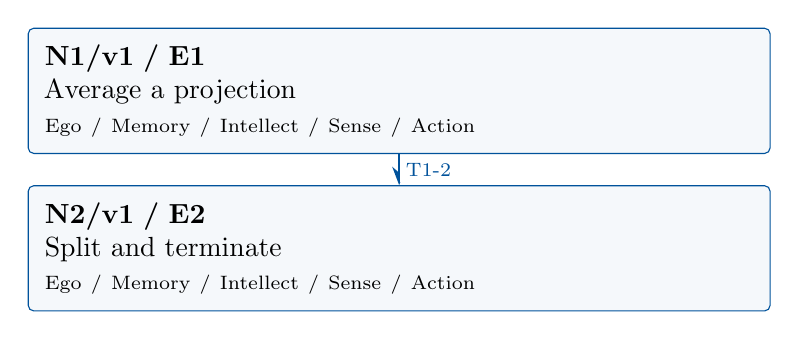
\begin{tikzpicture}[>=Stealth,x=1cm,y=1cm]

\node[mmnode,text width=9cm,minimum height=1.25cm] (N1) at (0,0.0) {\textbf{N1/v1 / E1}\\Average a projection\\{\scriptsize Ego / Memory / Intellect / Sense / Action}};

\node[mmnode,text width=9cm,minimum height=1.25cm] (N2) at (0,-2.0) {\textbf{N2/v1 / E2}\\Split and terminate\\{\scriptsize Ego / Memory / Intellect / Sense / Action}};

\draw[mmproof] (N1.south) -- node[mmnote,right] {T1-2} (N2.north);

\end{tikzpicture}\end{center}

Each box is one mathematical agent containing all five faculties. Blue
arrows carry the versioned exports listed below. The layout gives a
reading order; only drawn arrows assert dependencies. Diagnostic repair
is separate from the proof DAG.

\subsection{Versioned evidence-transfer ledger}

\begingroup\small\linespread{1.05}\selectfont

\Needspace{5\baselineskip}\field{T1-2: N1/E1/v1 to N2}{\(P=|G|^{-1}\sum_g\rho(g)p\rho(g)^{-1}\) is equivariant, has image
\(W\), and restricts to the identity on \(W\).}

\field{Receiving activity}{N2.1}

\field{Compatibility}{E1/v1 and finite \(\dim V\). Check: The recursive decomposition
terminates because each proper nonzero summand has smaller dimension.}

\endgroup

\clearpage\section{Agent roles and five-faculty activities}\begingroup\small\linespread{1.05}\selectfont\setlist{itemsep=1pt,topsep=2pt}

\subsection{N1/v1: Average a projection}

\field{Object and role}{Average \(\rho(g)p\rho(g)^{-1}\) to enforce equivariance without losing
the restriction to \(W\). \textbf{Local obligation:}
\(P=|G|^{-1}\sum_g\rho(g)p\rho(g)^{-1}\) is equivariant, has image
\(W\), and restricts to the identity on \(W\).}

\field{Inputs}{An invariant \(W\subset V\) and any linear projection \(p:V\to W\) with
\(p|_W=\mathrm{id}\).}

\mmfaculty{E}{Ego}{Publish E1/v1 only after establishing this obligation:
\(P=|G|^{-1}\sum_g\rho(g)p\rho(g)^{-1}\) is equivariant, has image
\(W\), and restricts to the identity on \(W\).}

\mmfaculty{M}{Memory}{An invariant \(W\subset V\) and any linear projection \(p:V\to W\) with
\(p|_W=\mathrm{id}\). Retain the stated assumptions and import versions.}

\mmfaculty{I}{Intellect}{Average \(\rho(g)p\rho(g)^{-1}\) to enforce equivariance without losing
the restriction to \(W\).}

\mmfaculty{S}{Sense}{Division by \(|G|\) must be legal, and each conjugate must still land in
\(W\).}

\mmfaculty{A}{Action}{Carry out activities N1.1--N1.2 below, retaining each calculation and
construction as evidence.}

\smallskip\noindent\textbf{Numbered mathematical activities}

\begin{enumerate}[label=N1.\arabic*,leftmargin=3.4em]

\item Choose a vector-space complement by extending a basis of \(W\), and let
\(p\) be its projection. Each conjugate of \(p\) lands in \(W\), since
\(W\) is invariant under every \(\rho(g)\). On \(w\in W\), that
conjugate sends \(w\) to itself. Thus the average \(P\) also maps into
\(W\) and is the identity there.

\item For \(h\in G\), conjugating \(P\) by \(\rho(h)\) replaces the index
\(g\) by \(hg\), a permutation of \(G\). Therefore \(P\) commutes with
\(\rho(h)\). Its restriction to its image is the identity, so \(P^2=P\)
and \(\operatorname{im}P=W\).

\end{enumerate}

\field{Export E1/v1}{\(P=|G|^{-1}\sum_g\rho(g)p\rho(g)^{-1}\) is equivariant, has image
\(W\), and restricts to the identity on \(W\).}

\field{Acceptance gate}{Division by \(|G|\) must be legal, and each conjugate must still land in
\(W\).}

\field{Targeted repair}{If \(p\) is assumed equivariant from basis extension alone, replace it
by the conjugation average and verify the reindexing. Withhold this
export and recheck its descendants after a versioned correction.}

\clearpage

\subsection{N2/v1: Split and terminate}

\field{Object and role}{Use the equivariant kernel as a complement, then induct on dimension.
\textbf{Local obligation:} \(V=W\oplus\ker P\) as representations, and
every such \(V\) is a finite direct sum of irreducibles.}

\field{Inputs}{E1/v1 and finite \(\dim V\). Incoming proof exports: E1/v1 at N2.1.}

\mmfaculty{E}{Ego}{Publish E2/v1 only after establishing this obligation:
\(V=W\oplus\ker P\) as representations, and every such \(V\) is a finite
direct sum of irreducibles.}

\mmfaculty{M}{Memory}{E1/v1 and finite \(\dim V\). Incoming proof exports: E1/v1 at N2.1.
Retain the stated assumptions and import versions.}

\mmfaculty{I}{Intellect}{Use the equivariant kernel as a complement, then induct on dimension.}

\mmfaculty{S}{Sense}{The recursive decomposition terminates because each proper nonzero
summand has smaller dimension.}

\mmfaculty{A}{Action}{Carry out activities N2.1--N2.2 below, retaining each calculation and
construction as evidence.}

\smallskip\noindent\textbf{Numbered mathematical activities}

\begin{enumerate}[label=N2.\arabic*,leftmargin=3.4em]

\item Every \(v\) decomposes as \(Pv+(v-Pv)\), with the first term in \(W\)
and the second in \(\ker P\). Their intersection is zero because
\(P|_W\) is the identity. If \(u\in\ker P\), then
\(P\rho(g)u=\rho(g)Pu=0\), so the complement is invariant.

\item For \(\dim V=0\) the decomposition is the empty sum. A nonzero
irreducible \(V\) is already one summand. Otherwise choose a proper
nonzero invariant \(W\), split it as above, and apply the induction
hypothesis to both summands of strictly smaller positive dimension. This
yields a finite irreducible decomposition.

\end{enumerate}

\field{Export E2/v1}{\(V=W\oplus\ker P\) as representations, and every such \(V\) is a finite
direct sum of irreducibles.}

\field{Acceptance gate}{The recursive decomposition terminates because each proper nonzero
summand has smaller dimension.}

\field{Targeted repair}{If repeated splitting is asserted to terminate without a measure, use
the strictly decreasing dimensions of the summands. Withhold this export
and recheck its descendants after a versioned correction.}

\endgroup\clearpage\section{Continuous mathematical proof}\label{sec:proof}

\subsection{N1 --- Average a projection}\label{n1-average-a-projection}

\begin{enumerate}
\def\labelenumi{\arabic{enumi}.}
\item
  \textbf{N1.1.} Choose a vector-space complement by extending a basis
  of \(W\), and let \(p\) be its projection. Each conjugate of \(p\)
  lands in \(W\), since \(W\) is invariant under every \(\rho(g)\). On
  \(w\in W\), that conjugate sends \(w\) to itself. Thus the average
  \(P\) also maps into \(W\) and is the identity there.
\item
  \textbf{N1.2.} For \(h\in G\), conjugating \(P\) by \(\rho(h)\)
  replaces the index \(g\) by \(hg\), a permutation of \(G\). Therefore
  \(P\) commutes with \(\rho(h)\). Its restriction to its image is the
  identity, so \(P^2=P\) and \(\operatorname{im}P=W\).
\end{enumerate}

\subsection{N2 --- Split and terminate}\label{n2-split-and-terminate}

\begin{enumerate}
\def\labelenumi{\arabic{enumi}.}
\item
  \textbf{N2.1.} Every \(v\) decomposes as \(Pv+(v-Pv)\), with the first
  term in \(W\) and the second in \(\ker P\). Their intersection is zero
  because \(P|_W\) is the identity. If \(u\in\ker P\), then
  \(P\rho(g)u=\rho(g)Pu=0\), so the complement is invariant.
\item
  \textbf{N2.2.} For \(\dim V=0\) the decomposition is the empty sum. A
  nonzero irreducible \(V\) is already one summand. Otherwise choose a
  proper nonzero invariant \(W\), split it as above, and apply the
  induction hypothesis to both summands of strictly smaller positive
  dimension. This yields a finite irreducible decomposition.
\end{enumerate}

\hfill$\square$

\section{Worked orchestration}

Let \(G=C_2\) act on \(k^2\) by swapping coordinates, with
\(\operatorname{char}k\ne2\). For \(W=k(1,1)\), start with
\(p(x,y)=(x,x)\). Averaging its two conjugates gives
\(P(x,y)=((x+y)/2,(x+y)/2)\). Its kernel is \(k(1,-1)\), yielding the
trivial and sign summands.

\subsection{Boundary and hypothesis audit}

Over \(\mathbb F_p\), let a generator of \(C_p\) act by \(T=I+N\) on a
two-dimensional space, where \(N e_2=e_1\) and \(N e_1=0\). Then
\(T^p=I\). The invariant line \(k e_1\) has no invariant complement: any
complementary line has a vector \(e_2+a e_1\), whose image differs by
\(e_1\) and cannot stay in that line. Here \(|G|=0\) in the field.

\section{Illustrative failure and repair}

The following is an authored diagnostic scenario. Changed assumptions
define a new contract; they do not retroactively prove the original
statement.

\subsection{Rejected argument, diagnosis, and correction}
\textbf{Rejected N1 candidate:} the same average proves complete
reducibility in every characteristic. \textbf{Sense:} the unipotent
\(C_p\) example contradicts the conclusion and \(1/|G|\) is undefined.
\textbf{Repair:} retain the stated invertibility assumption; no
averaging repair exists for that counterexample under the broader claim.
Recheck the complement and recursive decomposition with the correct
field contract.

\subsection{Publication and reuse}
The corrected export retains its explicit assumptions. A hypothetical
revision receives a new version, and each consuming activity is
rechecked; this scenario is not a recorded runtime event. \textbf{Next
direction:} Use invariant complements to decompose finite-group
representations before character calculations; this does not itself
prove the corresponding claim for arbitrary Lie algebras.

\par\medskip\begingroup\small\linespread{1.0}\selectfont\noindent\textbf{Provenance.} This authored proof is complete relative to its declared imports. Reuse
each export with its assumptions, proof, and version. The original
Markdown remains available for comparison.
\par\endgroup

\par\smallskip\begingroup\small\linespread{1.0}\selectfont\noindent\textbf{Further reading.} \href{https://math.mit.edu/~etingof/reprbook.pdf}{Etingof and
collaborators, Introduction to Representation Theory}, sections on
representations, characters, and \(\mathfrak{sl}_2\);
\href{https://ocw.mit.edu/courses/18-745-lie-groups-and-lie-algebras-i-fall-2020/lists/lecture-notes/}{MIT
Lie Groups and Lie Algebras I lecture notes} for solvable Lie algebras.\par\endgroup

\end{document}
